
\subsection{Types and Functions}

In the LHC machine, there are various accelerator magnets which can be divided into three main groups based on their function~\cite{cern_main_webpage}: 
\begin{enumerate}
    \item Dipole magnets. They apply a centripetal Lorentz force to moving particle beams in order to maintain them in the curvature of a 27-km ring. There are 1232 dipoles in the LHC.
    \item Main quadrupole magnets. They constrain the width and the height of a particle beam in order to maintain them inside of a vacuum chamber inside the LHC magnet. There are 392 such magnets inside the LHC.
    \item Corrector magnets. They aim at correcting imperfections in the field quality created in the aforementioned magnets. Some of the examples of such magnets are: dipole orbit correctors, quadrupoles and skew quadrupoles, sextu-, octu-, deca- or dodecapoles. 
\end{enumerate}

Fig.~\ref{fig:cross_section_lhc_main_dipole} presents the cross-section of the main LHC dipole. The particle beam is travelling inside of a vacuum chamber surrounded by a coil composed of multiple turns of a~superconducting wire. During the operation of the machine, Lorentz forces are exerted on the coil. Therefore, the coils are usually clamped with pre-stressed steel collars holding them together with a sufficient precision. The collars are surrounded by a concentrically mounted iron yoke. The iron yoke increases the central magnetic field that directs a travelling beam and reduces the magnetic energy stored in the coil.

\begin{figure}[H]
    \centering
    \begin{tikzpicture}
    \node at (0,0) {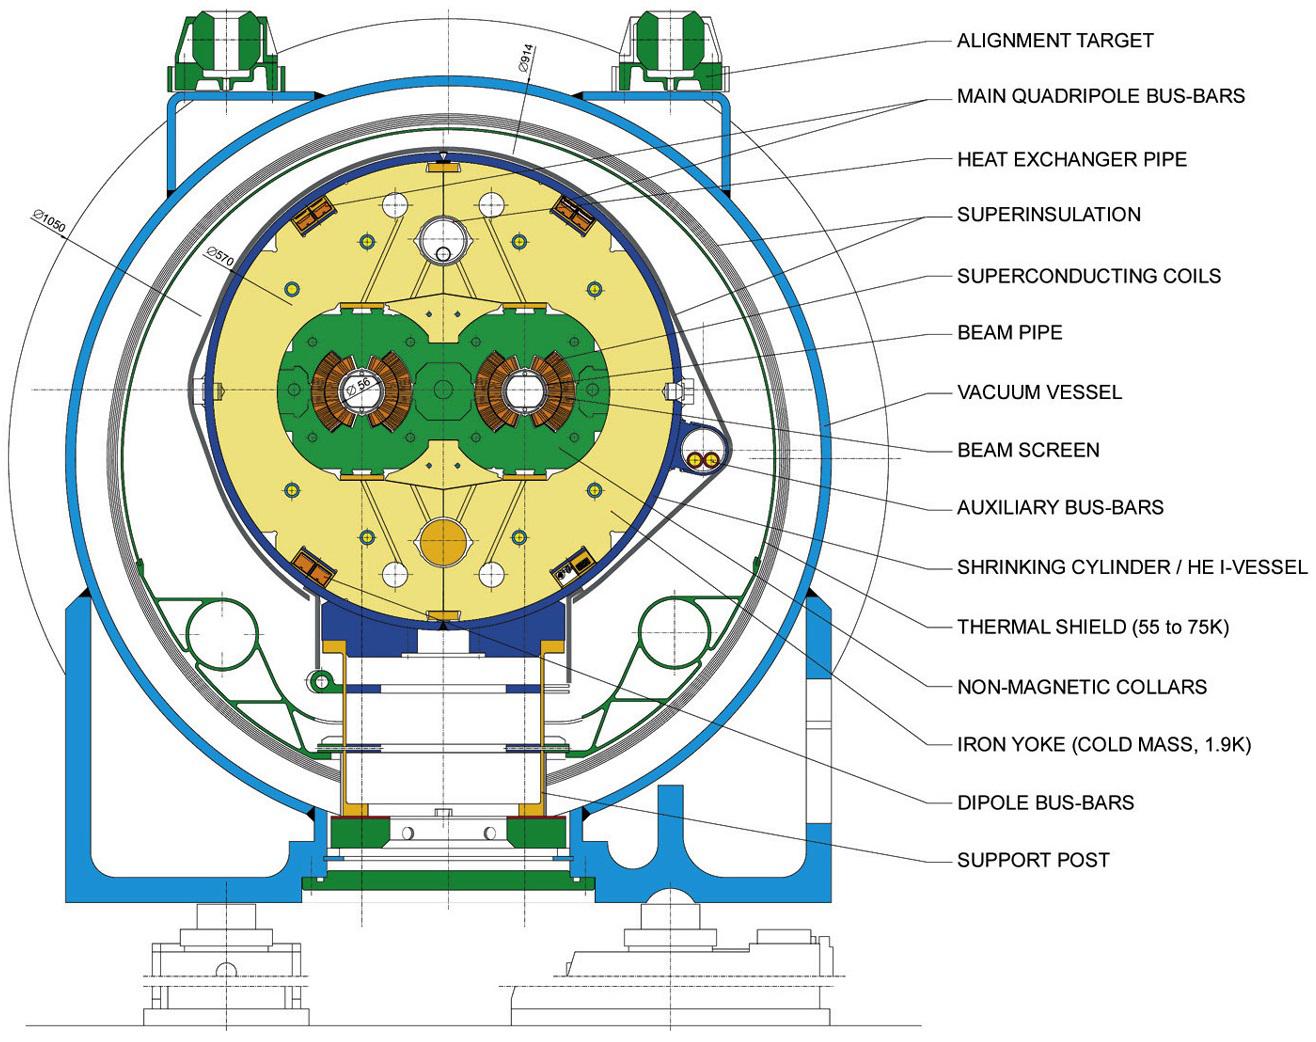
\includegraphics[width=.5\textwidth]{sections/introduction/figures/LHC_main_dipole_cross_section.png}};
    \end{tikzpicture}
    \caption{Cross-section of the LHC main dipole magnet with description of main components.~\cite{lhc_main_dipole_cross_section}.}
    \label{fig:cross_section_lhc_main_dipole}
\end{figure}

\subsection{Quench Protection}

When a quench occurs at operating conditions of a superconducting magnet, it ought to be detected in the shortest possible time. Otherwise, it may lead to an irreversible destruction of the machine. As soon as the quench is detected, the power supply is cut off and the magneto-electric energy stored is discharged. Basically, the energy should be either deposited in the coil or extracted from the magnet. The quench protection can be active or passive. The active systems use additional protection devices that improve the discharge efficiency, i.e. the current drop is quicker. There are four main active protection systems: 

\begin{enumerate}
	\item Energy extraction,
	\item Quench heaters,
	\item Couple-Loss-Induced-Quench (CLIQ) system. 
\end{enumerate}

In case of an energy extraction, a part of the energy stored in a magnet is discharged in an external dump resistor connected in series with the machine. Such a system is available as soon as the magnet is disconnected from its power supply and it limits the energy deposited directly in the coil. The magnet recovers faster to its operating conditions because it requires less cooling power after the discharge process. The extraction system usually cannot discharge the entire energy because its resistance is limited by the maximum voltage allowed across the magnet terminals. At cryogenic temperatures, the electrical permeability of the insulation between different windings of the coil is reduced. Therefore, the increase of voltage across the coil may lead to a short-circuit inside of a magnet~\cite{salmiquenchheateroptimization}. 

Quench heaters are resistive strips installed along the coils in a close contact with the windings. The heaters have an external power supply usually based on a charged capacitor. When a quench is detected, the heaters are fired. Due to the firing of the protection system, the cables, being in a close contact with the heaters, quench over a longer distance. A~larger resistive volume is created in the magnet and the discharge occurs faster. Moreover, the temperature in the quenched coil is also more uniformly distributed without the formation of one distinct hot spot. The quench heaters have an external power supply independent of the superconducting coils. Therefore, they must be electrically insulated from the windings. In fact, the electrical insulation is a thermal barrier causing a delay between the moment when the heaters are fired and the time when the coil quenches. This delay is a characteristic feature of a quench heating system. The drawbacks of the quench heaters are as follows~\cite{salmiquenchheateroptimization}: 

\begin{itemize}
	\item The heaters are additional elements placed inside of a compact structure of a magnet. Their arrangement leads to a certain pre-stress of the coils which has to be taken into account at the stage of a magnet design.
	\item The electro-thermal insulation between the heaters and the coil must be thoroughly analysed with respect to the possible short circuits and the delay of a quench firing system.
	\item There is no possibility to replace quench heating strips of the magnet once they are installed. Therefore, the maintenance of this system is limited in a long-term of a machine operation. 
\end{itemize}

Coupling-Loss-Induced-Quench system aims at generating current oscillations in the superconducting windings to create a fast change of a magnetic field. According to the Faraday’s law, the variation of a magnetic field in time induces eddy currents in an electrical conductor, called AC-losses. According to~\cite{ravaioli_cliq_phd_thesis}, the CLIQ induces quench faster than quench heaters. It is a backup solution for currently developed high energy accelerator magnets made of $\text{Nb}_3 \text{Sn}$ for the High-Luminosity LHC project. 

The AC-losses also occur in the coil during a standard discharge due to the drop of current when no CLIQ unit is implemented. The change of current induces the change of a magnetic field, being a source of eddy currents. Therefore, if the current drops sufficiently fast, the eddy currents may induce a quench in the parts of a coil which remain superconductive. This phenomenon is called a “quench back”.

A superconducting magnet can also be "self-protected" meaning that no active quench protection devices are installed. This is the simplest and the cheapest solution. The self-protectability is applicable in magnets characterised by a relatively low current densities and, therefore, low magnetic fields. A low level of the stored energy allows the magnet to limit the temperature rise during the discharge. 
